% C2. El reto: train en toda Bogotá, test en Chapinero
\begin{frame}{El reto: predecir donde casi no hay datos}
  \begin{columns}[c]
    \begin{column}{0.5\textwidth}\centering
      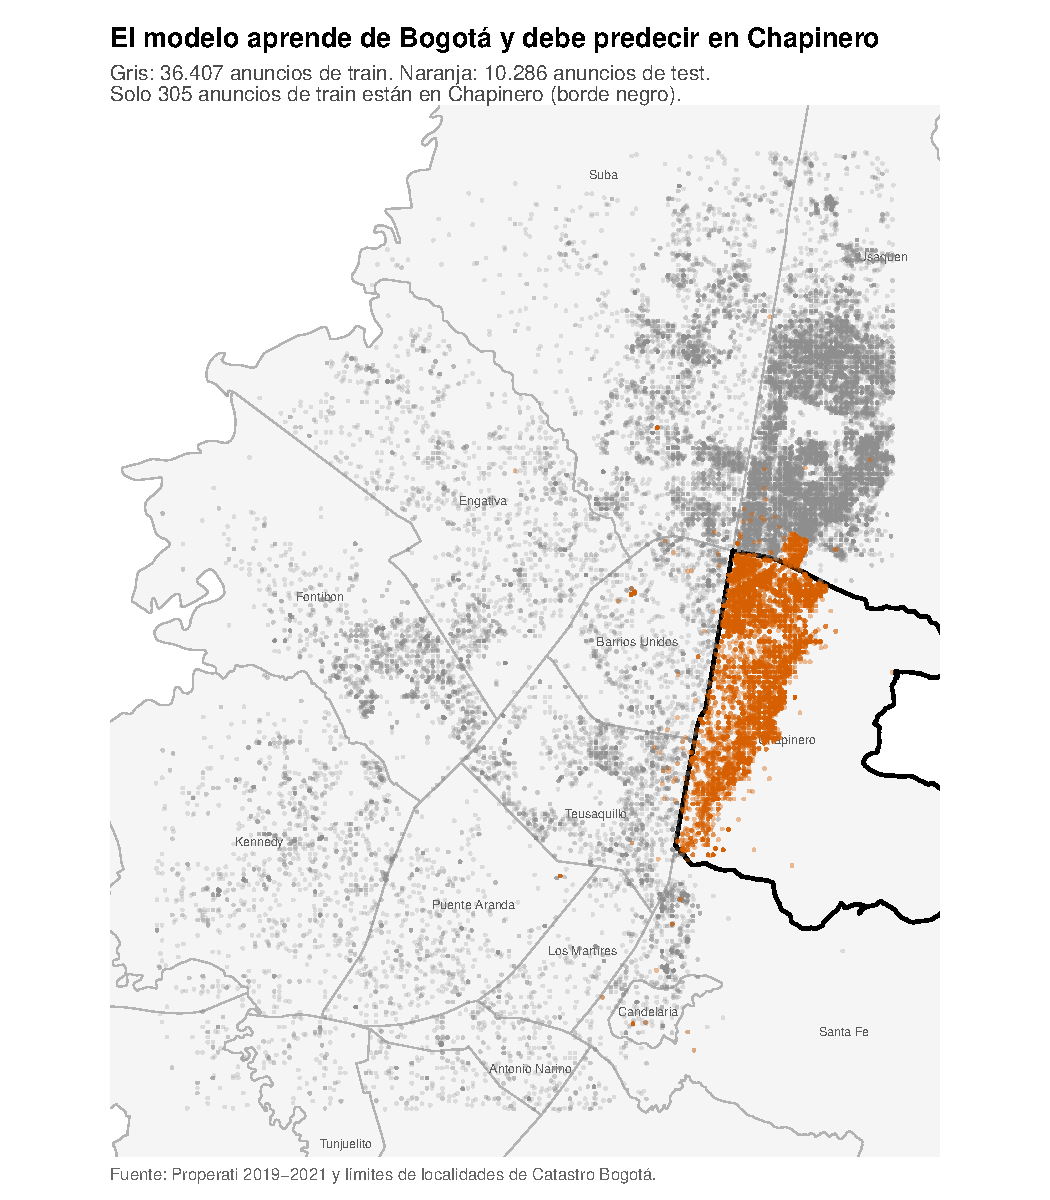
\includegraphics[height=0.82\textheight]{mapa_01_train_test.pdf}
    \end{column}
    \begin{column}{0.45\textwidth}
      \cifra[\linewidth]{\ntrain}{anuncios de train en toda Bogotá}\\[1.2em]
      \cifra[\linewidth]{\nchaptrain}{de ellos en Chapinero}\\[1.2em]
      \cifra[\linewidth]{\pcttestchap}{de los \ntest{} anuncios de test están en Chapinero}
    \end{column}
  \end{columns}
  \note{La empresa quiere comprar en Chapinero, pero los datos para aprender son de toda la ciudad. El modelo tiene que extrapolar: aprender en Suba, Kennedy o Usaquén y predecir en Chapinero. Por eso la validación cruzada aleatoria no basta, y por eso usamos validación espacial.}
\end{frame}
